\documentclass[11pt,a4paper]{article}
\usepackage{cite}
\usepackage{color}
\usepackage{graphicx}
\usepackage{amsmath}
\usepackage[margin=1in]{geometry}

\title{The DJH Inertial Navigation System Package}
\author{David Hanley}

\begin{document}
\maketitle

\begin{abstract}
In this document, we cover the details of the Inertial Navigation System: the various classes and their relationship to each other, future work, and related references for inertial navigation.
\end{abstract}

\section{Introduction: System Overview}

As shown by Figure \ref{fig:UML}, the DJH Inertial Navigation System package is composed of C++ classes configured into three related layers. The first layer is the Interface Layer, which is composed of the djh\_ins class. This is the only class an individual using the package will interact with. Initializing this function, a user sets a gravity model, IMU model, and chooses the method of INS integration (or preintegration). The djh\_ins class is composed of a set of classes that correct IMU measurements using the IMU model and subsequently integrate (or preintegrate) measurements. This set of classes makes up the Integration Layer. The Integrator class within the Integration Layer is also composed of a series of classes for using JPL-style quaternions, using generic rigid body dynamics, and using a given model of gravity. This last set of classes makes up the Model Layer of the package.

This package assumes that Eigen is already installed on the system. See the Wiki page on the DJH INS github for installation instructions and examples of usage.

\begin{figure}[htp]
	\centering
	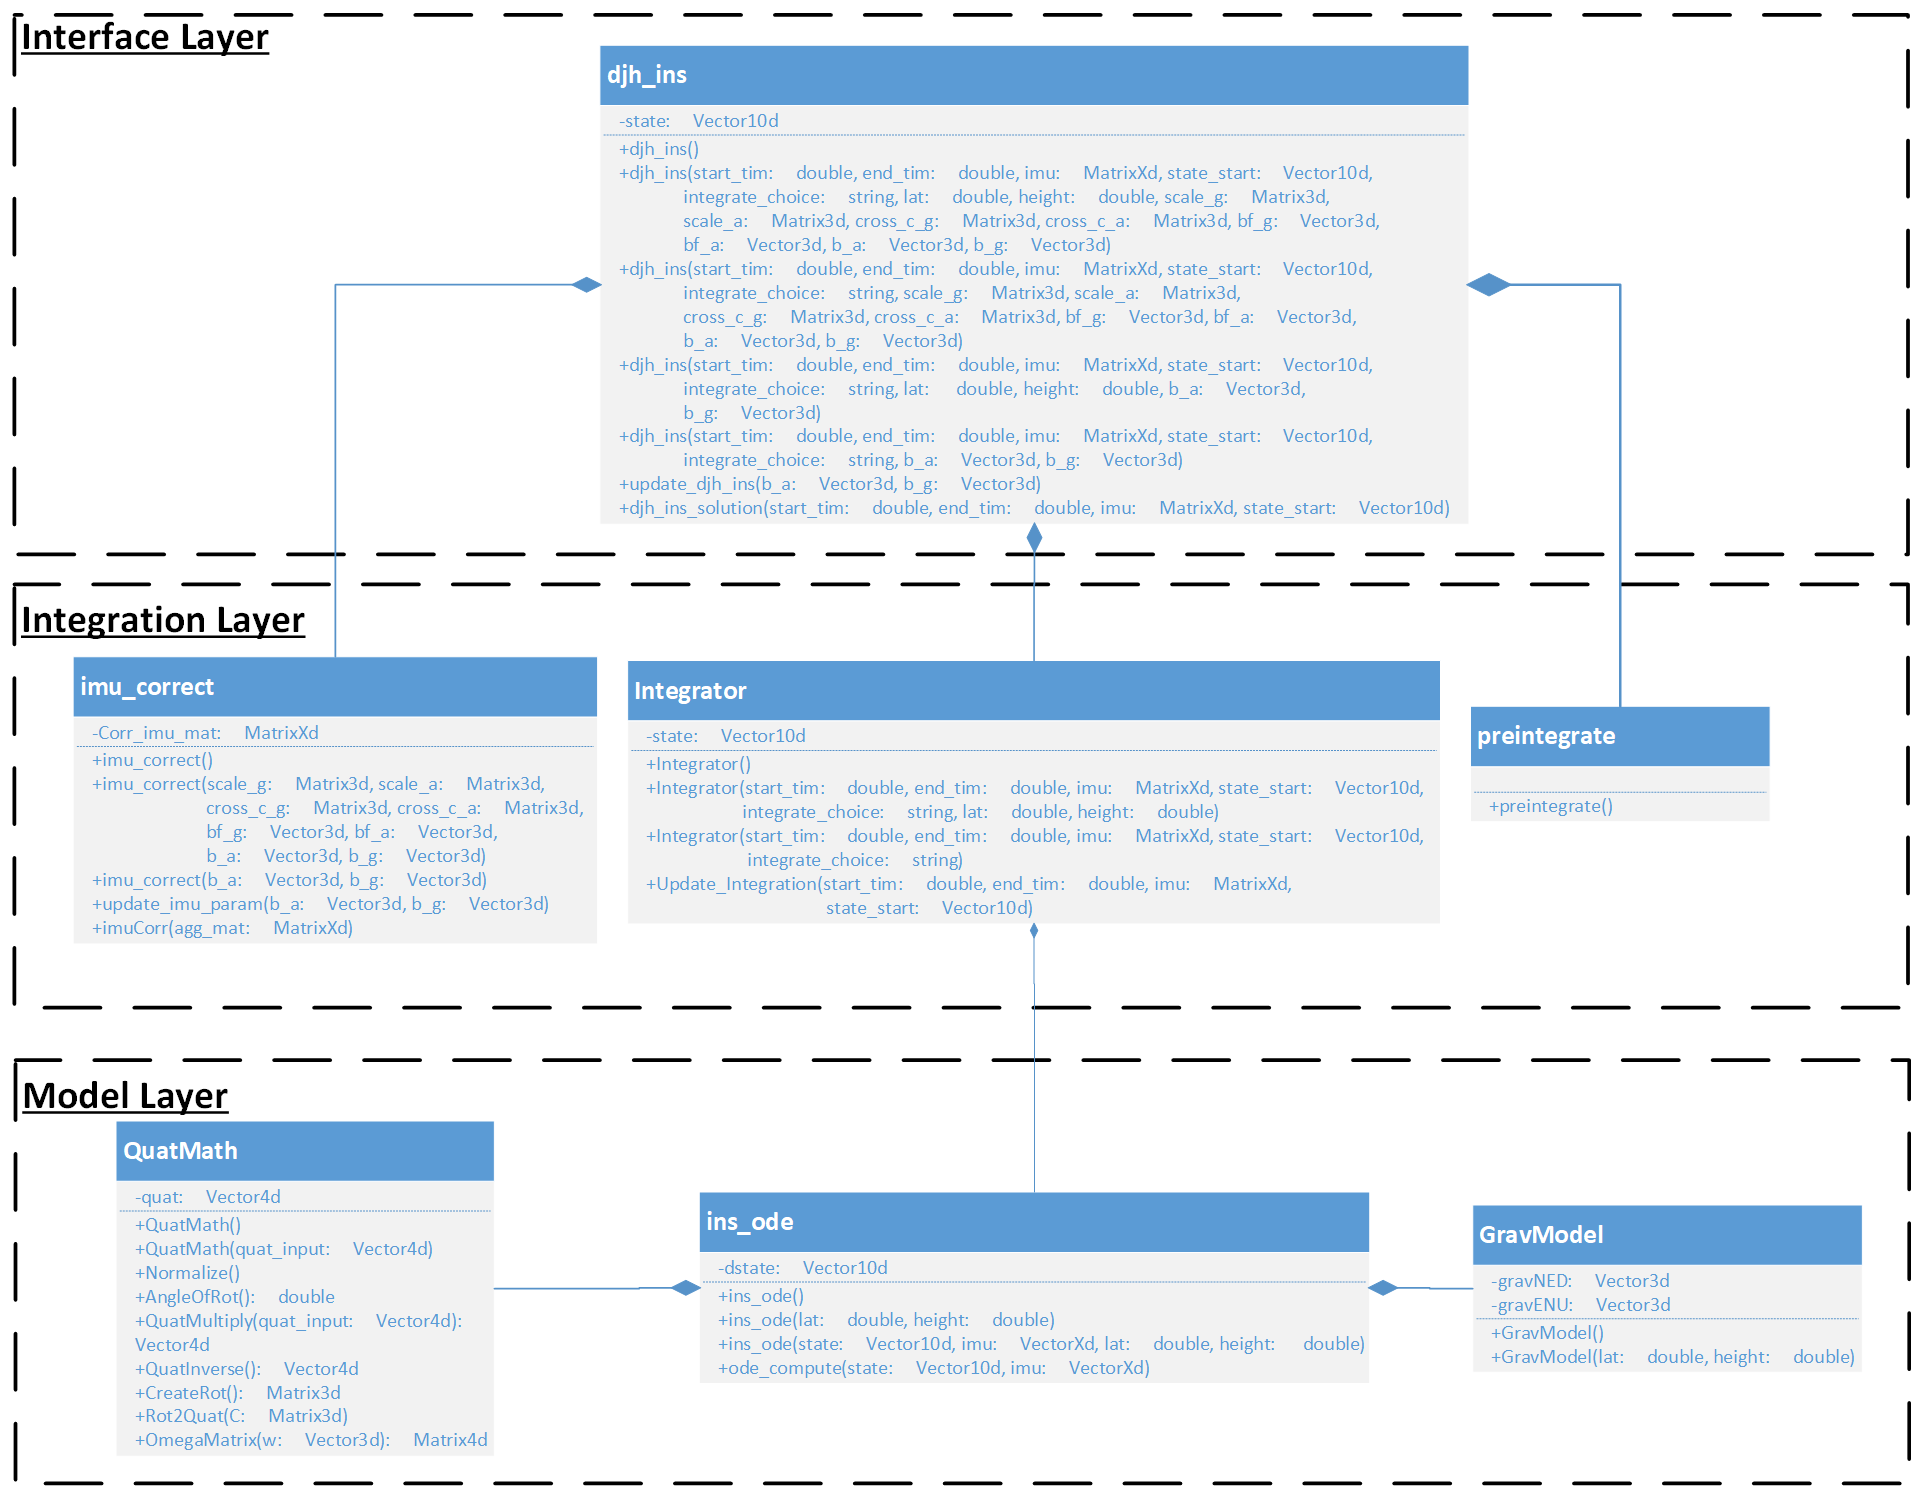
\includegraphics[scale=0.4]{pictures/UMLofdjh_ins}
	\caption{This UML diagram of the DJH INS package shows that classes in the system are broken into three layers: the interface layer, the integration layer, and the model layer. When using the package, users only use the interface layer and its class.}
	\label{fig:UML}
\end{figure}

\section{Individual Class Descriptions}

Note: italicized variables and data types indicate optional inputs.

	\subsection{QuatMath}
	QuatMath is a quaternion math class for the INS package. This class contains quaternion math functions using the JPL quaternion convention. To the best of our knowledge, the Eigen library uses the Hamilton convention for quaternions. So we do not use that functionality.
	\begin{itemize}
		\item[\textbf{Attribute:}] quat:  Vector4d
		
		Public JPL Quaternion variable
		\begin{equation*}
			quat = \left[q_x, q_y, q_z, q_w\right]^T
		\end{equation*}
		\item[\textbf{Constructor:}] QuatMath(\textit{Vector4d quat\_input})

		quat\_input = JPL input quaternion of the form $\left[q_x, q_y, q_z, q_w\right]^T$
		
		\item[\textbf{Function:}] Normalize()
		
		This function ensures that the class' quaternion has a norm of 1.
		
		\item[\textbf{Function:}] AngleOfRot()
		
		Compute the angle of rotation of the class' quaternion.
		
		Output: the angle of rotation in radians.
		
		\item[\textbf{Function:}] QuatMultiply(Vector4d quat\_input):  Vector4d
		
		Multiply the class quaternion (q) by an input quaternion (p) in the form q*p
		
		quat\_input = JPL input quaternion of the form 
		
		Output: Output quaternion from multiplication q*p
		
		\item[\textbf{Function:}] QuatInverse():  Vector4d
		
		Compute and output the inverse of the class' quaternion.
		
		Output: the inverse of the class' quaternion
		
		\item[\textbf{Function:}] CreateRot():  Matrix3d
		
		Output rotation matrix of the class' quaternion
		
		Output: the 3$\times$3 rotation matrix represented by the class' quaternion
		
		\item[\textbf{Function:}] Rot2Quat(Matrix3d C)
		
		Assigns the class' quaternion to be equivalent to a rotation matrix input
		
		C = a rotation matrix to be converted to a quaternion
		
		\item[\textbf{Function:}] OmegaMatrix(Vector3d w):  Matrix 4d
		
		This function computes a 4$\times$4 matrix of angular velocities from a vector of angular velocities. This matrix can be used in a quaternion's equation of motion.
		
		w = a three element vector of angular velocity $\left[\begin{array}{ccc}w_x & w_y & w_z\end{array}\right]^T$.
		
		Output: a 4$\times$4 matrix of angular velocities that can be used in quaternion equations of motion.
	\end{itemize}
	
	\subsection{ins\_ode}
	
	ins\_ode is a class expressing the ordinary differential equations for a generic rigid body as used in an inertial navigation system.
	
	\begin{itemize}
		\item[\textbf{Attribute:}] dstate:  Vector10d
		
		State time derivative: $\left[\begin{array}{ccc}quat & position & velocity\end{array}\right]$
		
		\item[\textbf{Constructor:}] ins\_ode(\textit{Vector10d state, VectorXd imu, double lat, double height})
		
		state = $\left[\begin{array}{ccc}quat & position & velocity\end{array}\right]$ 
		
        imu = $\left[\begin{array}{cc} accel & gyros\end{array}\right]$
        
        lat = latitude of sensor (in radians) for gravity calculation
        
        height = height of sensor (in meters) for gravity calculation
        
        This class can be constructed using no inputs, using only latitude and height, or using all the optional inputs.
        
        \item[\textbf{Function:}] ode\_compute(\textit{Vector10d state, VectorXd imu})
        
        This function updates the state derivatives.
	\end{itemize}
	
	\subsection{GravModel}
	
	\begin{itemize}
		\item[\textbf{Attribute:}] gravNED:  Vector3d
		
		The NED (North, East, Down) gravity vector		
		
		\item[\textbf{Attribute:}] gravENU:  Vector3d
		
		The ENU (East, North, Up) gravity vector
		
		\item[\textbf{Constructor:}] GravModel(\textit{double lat, double height})
		
		lat = latitude (in radians) of current sensor location
        
        height = altitude (in meters) of current sensor location
	\end{itemize}

	\subsection{preintegrate}

	\begin{itemize}
		\item[\textbf{Constructor:}] preintegrate()
	\end{itemize}
	
	\subsection{imu\_correct}
	
	\begin{itemize}
		\item[\textbf{Attribute:}] Corr\_imu\_mat:  MatrixXd
		
		Aggregated IMU matrix adjusted to eliminate IMU errors.
		
		Matrix is of the form:
		
		$\left[\begin{array}{ccc}
					time_1 & accel & gyro \\
					time_2 & accel & gyro \\
					...    & ...   & ...  \\	
		\end{array}\right]$
		
		\item[\textbf{Constructor:}] imu\_correct(\textit{Matrix3d scale\_g, Matrix3d scale\_a, Matrix3d cross\_c\_g, Matrix3d cross\_c\_a, Vector3d bf\_g, Vector3d bf\_a, Vector3d b\_a, Vector3d b\_g});
		
		scale\_g = scale factor errors for IMU gyroscopes

        scale\_a = scale factor errors for IMU accelerometers

        cross\_c\_g = cross coupling errors for IMU gyroscopes

        cross\_c\_a = cross coupling errors for IMU accelerometers

        bf\_g = fixed gyroscope biases

        bf\_a = fixed accelerometer biases

        b\_a = accelerometer biases estimated online

        b\_g = gyroscope biases estimated online
        
        This class can be constructed using no inputs, online estimated accelerometer and gyroscope biases, or using all the optional inputs.

	\item[\textbf{Function:}] update\_imu\_param(Vector3d b\_a, Vector3d b\_g)

		Update the IMU error components
		
        b\_a = accelerometer biases estimated online

        b\_g = gyroscope biases estimated online
        
	\item[\textbf{Function:}] imuCorr(MatrixXd agg\_mat)
        
		imuCorr accepts an aggregated n-by-7 IMU matrix and corrects the IMU measurements for fixed scale, bias, and cross-coupling factors. It then adds a bias estimated online.        
        
        agg\_mat = Aggregated IMU matrix of the form
        
        $\left[\begin{array}{ccc}
					time_1 & accel & gyro \\
					time_2 & accel & gyro \\
					...    & ...   & ...  \\	
		\end{array}\right]$
	\end{itemize}
	
	\subsection{Integrator}
	
	\begin{itemize}
		\item[\textbf{Attributes:}] state:  Vector10d
		
		This is the 10 dimensional INS State Estimate 
		
		$\left[\begin{array}{ccc}quat & position & velocity\end{array}\right]^T$
		
		\item[\textbf{Constructor:}] Integrator(\textit{double start\_tim, double end\_tim, MatrixXd imu, Vector10d state\_start, string integrate\_choice, double lat, double height})

		start\_tim = start time in seconds (presumably a Unix time)

        end\_tim = end time in seconds (presumable a Unix time)

        imu = IMU measurement matrix of the form
        
		$\left[\begin{array}{ccc}
					time_1 & accel & gyro \\
					time_2 & accel & gyro \\
					...    & ...   & ...  \\	
		\end{array}\right]$
		
		And we assume entries are in chronological order (i.e. time\_1 $<$ time\_2 $<$ ...)
        
        state\_start = starting state prior to integration (10 elements: quaternion, position, velocity)
        
        integration\_choice = a string selecting either "Euler", "Heun", "RK4", or "Savage" methods
        
        lat = latitude of the starting point (for gravity model)
        height = height of the starting point above sea level (for gravity model)		
		
		This class can be constructed using no inputs, all the optional inputs, or using start time, end time, imu data, the starting state and the choice of integrator.
		
		\item[\textbf{Function:}] Update\_Integration(double start\_tim, double end\_tim, MatrixXd imu, Vector10d state\_start)
					
		Update\_Integration updates the INS solution given a start and end time, IMU measurements, and a starting state estimate.
		
		start\_tim = start time in seconds (presumably a Unix time)
		
        end\_tim = end time in seconds (presumably a Unix time)
        
        imu = IMU measurement matrix of the form

		$\left[\begin{array}{ccc}
					time_1 & accel & gyro \\
					time_2 & accel & gyro \\
					...    & ...   & ...  \\	
		\end{array}\right]$
        
        And we assume entries are in chronological order (i.e. time\_1 $<$ time\_2 $<$ ...)
        
        state\_start = starting state prior to integration (10 elements: quaternion, position, velocity)
	\end{itemize}

	\subsection{djh\_ins}

	\begin{itemize}
		\item[\textbf{Attributes:}] state:  Vector10d

		This is the 10 dimensional INS State Estimate 
		
		$\left[\begin{array}{ccc}quat & position & velocity\end{array}\right]^T$
		
		\item[\textbf{Constructor:}] djh\_ins(\textit{double start\_tim, double end\_tim, MatrixXd imu, Vector10d state\_start, string integrate\_choice, double lat, double height, Matrix3d scale\_g, Matrix3d scale\_a, Matrix3d cross\_c\_g, Matrix3d cross\_c\_a, Vector3d bf\_g, Vector3d bf\_a, Vector3d b\_a, Vector3d b\_g})
		
		start\_tim = start time in seconds (presumably a Unix time)

        end\_tim = end time in seconds (presumable a Unix time)

        imu = IMU measurement matrix of the form
        
		$\left[\begin{array}{ccc}
					time_1 & accel & gyro \\
					time_2 & accel & gyro \\
					...    & ...   & ...  \\	
		\end{array}\right]$
        
        And we assume entries are in chronological order (i.e. time\_1 $<$ time\_2 $<$ ...)
        
        state\_start = starting state prior to integration (10 elements: quaternion, position, velocity)

        integration\_choice = a string selecting either "Euler", "Heun", "RK4", or "Savage" methods
        
        lat = latitude of the starting point (for gravity model)
        
        height = height of the starting point above sea level (for gravity model)
        
        scale\_g = scale factor errors for IMU gyroscopes

        scale\_a = scale factor errors for IMU accelerometers

        cross\_c\_g = cross coupling errors for IMU gyroscopes

        cross\_c\_a = cross coupling errors for IMU accelerometers

        bf\_g = fixed gyroscope biases
        
        bf\_a = fixed accelerometer biases

        b\_a = accelerometer biases estimated online
        
        b\_g = gyroscope biases estimated online
        
        This class can be constructed using (1)no inputs, (2)all the optional inputs, (3)using start time, end time, IMU data, starting state, the choice of integrator, the scale factor errors for IMU gyroscopes and accelerometers, the cross coupling errors for IMU gyroscopes and accelerometers, the fixed biases for gyroscopes and acclerometers, and online estimated accelerometer and gyroscope biases, (4)using start time, end time, IMU data, starting state, the choice of integrator, the latitude, the height, and accelerometer and gyroscope biases estimated online, (5)using start time, end time, IMU data, starting state, the choice of integrator, and accelerometer and gyroscope biases estimated online.
        
        \item[\textbf{Function:}] update\_djh\_ins(Vector3d b\_a, Vector3d b\_g)
        
        Update IMU error components
        
        b\_a = accelerometer biases estimated online
        
        b\_g = gyroscope biases estimated online
        
        \item[\textbf{Function:}] djh\_ins\_solution(double start\_tim, double end\_tim, MatrixXd imu, Vector10d state\_start)
        
        Correct IMU data and generate updated state estimate using integration
        
        start\_tim = start time in seconds (presumably a Unix time)
        
        end\_tim = end time in seconds (presumably a Unix time)
        
        imu = IMU measurement matrix of the form
		
		$\left[\begin{array}{ccc}
					time_1 & accel & gyro \\
					time_2 & accel & gyro \\
					...    & ...   & ...  \\	
		\end{array}\right]$
        
        And we assume entries are in chronological order (i.e. time\_1 $<$ time\_2 $<$ ...)
        
        state\_start = starting state prior to integration (10 elements: quaternion, position, velocity)
	\end{itemize}

\section{Future Work}

\begin{itemize}
	\item
	Include IMU integration described by Paul G. Savage \cite{Savage:1998,Savagep2:1998}
	\item
	Include IMU preintegration computation as described by Kevin Eckenhoff, Patrick Geneva, and Guoquan Huang \cite{Eckenhoff:2016}
	
	\item 
	Provide as unit tests, the scenarios for testing INS systems described by Paul G. Savage \cite{Savage:2009}
\end{itemize}

\section{Related References}

General information about numerical integration methods can be found in \cite{Heath:2002}. For an overview of inertial measurement units, the technology involved, and a look at inertial navigation systems see the work of Titterton and Weston \cite{Titterton:2004}. Paul G. Savage's work on inertial navigation has been and appears to remain the current state of the art in the field \cite{Savage:1998,Savagep2:1998,Savage:2007,Savagep2:2007,Savage:2009}. For information about JPL-style quaternions see \cite{Barfoot:2011,Trawny:2005,NAIF:2003,Shuster:1993}. Information about preintegration (and its application to visual-inertial odometry) is described in \cite{Forster:2017,Forster:2015,Eckenhoff:2016}.

\bibliographystyle{IEEEtran}
\bibliography{IEEEabrv,references}

\end{document}